\section{Evaluation}
\label{sec:evaluation}
%ours, RPL + ContikiMAC, MiCMAC
The performance of MCRP is compared against the standard RPL with ContikiMAC on a single channel.

\subsection{Experimental Setup}
%//methodology? key metrics?
We evaluate the protocol in the  Cooja simulated environment with emulation of TMote sky nodes that feature the CC2420 transceiver, a 802.15.4 radio. The nodes run on IPv6, using UDP with standard RPL and 6LoWPAN protocols. The network consists of 16 nodes are used to run the simulation where we have 1 border router node, 1 interference node, and 14 duty cycled nodes that act as UDP clients to send packets to LPBR. RPL border router is used as LPBR in order to move most processing decisions on a PC as it has more RAM and better processing capabilities than a sensor. TelosB has limited RAM and ROM of 10K bytes and 48K bytes of flash memory. By using a border router, this allows channel changing to be decided in real time without draining the memory and battery on a sensor. The border router also acts as the root of the tree.

We simulated a controlled interference node that generates semi-periodic bursty interference to resemble a simplified WiFi or Bluetooth transmitter on channel 22. The interference model that we use is described in \cite{Boano:2010:MSM:2127940.2127963}. The interference has two states, a clear state and an interference state. In the clear state the interferer produces no packets and stays in this state for between $9/16$ seconds and $15/16$ seconds. In the interference state, the interference node generates packets for a time that is uniformly distributed between $3/4 * \emph{clear\textunderscore time}$ and $5/4 * \emph{clear\textunderscore time}$ where \emph{clear\textunderscore time} refers to the rate of interference (see later). We use single channel interference in our simulation to show our hypothesis that multiple channels can help avoid interference.  We consider a scenario where an RPL system is subject to interference on its channel after set up has successfully completed so the RPL set up is allowed to complete before
interference begins.

%We plan to run our protocol on the testbed as our future work to test on several interference channels.


%//why 1 channel? use a single channel interference "to show our hypothesis that multiple channels can help avoid interference we consider a scenario where an RPL system is subject to interference on its channel after set up has successfully completed"


We evaluate MCRP using an end-to-end packet delivery performance metric. The transmission success rate is calculated from the sender to the receiver over multiple hops. We also look at the loss over time to observe the protocol performance in the presence of interference.

%//be more clear about interference model; when it switches on, what is the experimental setup - systematic description of all stages and why. DON'T MENTION PROBLEMS!

We run the simulation for a duration of 70 minutes to send 700 packets. When the nodes are switched on for the first time, all nodes are initialised to channel 26 by default. RPl is allowed five minutes to set up (which is ample time). RPL topology is formed in a minute. We wait for another 4 minutes to allow trickle timer to doubles the interval length so that RPL control messages are less frequently invoke. We then let our multichannel protocol runs for 10 minutes. In our 15 nodes simulation, our protocol takes 7-8 minutes to run the channel change set up. We allow another 2 minutes wait time if channel changes retransmission happen. In a single channel simulation, all the nodes are changed to channel 22 after 5 minutes of RPL set up time. This allows RPL to have enough time to discover all nodes to form an optimised topology. The topology formation does not formed completely if the interference node interferes from the beginning. The interference node starts sending packets to interfere after 3 minutes the system is switched on so that the interference channel is involve in the channel changes decision. We proved that our protocol tries to avoid from changing to the interference channel through time out and probing failures. After 15 minutes, the client nodes will send a normal packet periodically every 30-60 seconds to LPBR. This is done in order to avoid collision of the nodes sending at the same time. The simulation is repeated 10 times.

%We evaluate multichannel RPL variant using three performance metrics: end to end packet delivery, latency and duty cycle. In end to end packet delivery, the transmission success rate is calculated from the sender to the receiver over multiple hops. The latency, time difference from sending to receiving is also calculated based on Cooja log time. Contiki's energy profiler is used to measure the duty cycle where the radio usage time in the total run is calculated.


\subsection{Effect of Multi-channel}
%//with existings - better? worse? what about RAM, ROM used?


\begin{figure}
\centering
\subfigure[Mild Interference]{\label{fig:mild}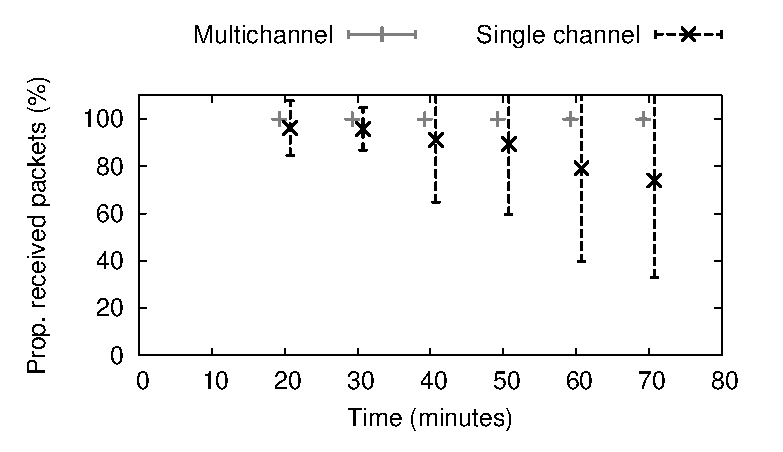
\includegraphics[width=0.45\textwidth]{experiments/mild.eps}}                
\subfigure[Moderate Interference]{\label{fig:mod}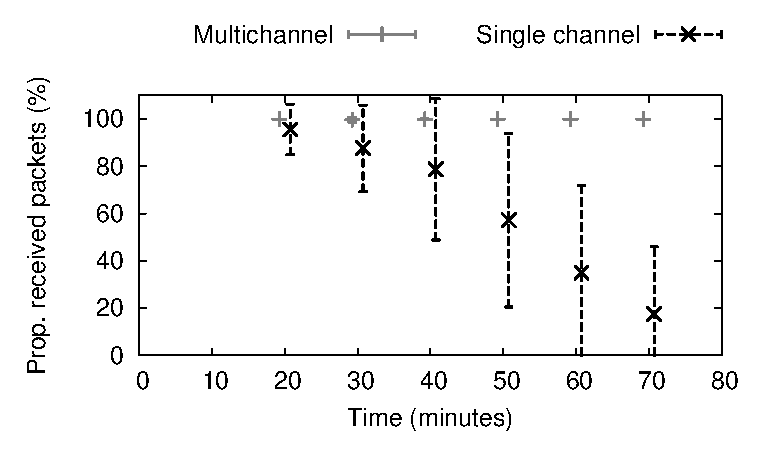
\includegraphics[width=0.45\textwidth]{experiments/moderate.eps}}
\subfigure[Extreme Interference]{\label{fig:extreme}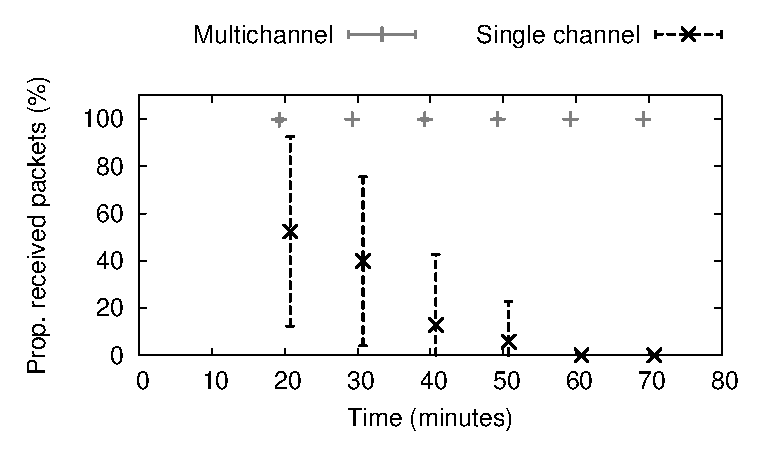
\includegraphics[width=0.45\textwidth]{experiments/extreme.eps}}
\caption{Level of packet loss for mild, moderate and extreme interference levels using single and multi-channel}
\label{fig:interference}
\end{figure}

We vary the interference rate, which is referred to as \emph{clear\textunderscore time} in \cite{Boano:2010:MSM:2127940.2127963} to 100\% (no interference), 75\% (mild), 50\% (moderate) and 25\% (extreme) where the percentage is the ratio of the time the channel is cleared from interference. The test is done to evaluate our protocol behaviour in different interference rate and to compare the result with a single channel case. Figure \ref{fig:interference} shows the mean results from ten simulation runs in each scenario and the error bars represent the standard deviation. We observed that during high interference and moderate interference, when the LPBR generates a random two hop channel for a node to change into, the receiving node will probe on the channel. It will either time out or the probing messages received are less than a threshold that allows for the node to change it's listening channel to the new channel. This is as expected as our protocol checks the channel each time before deciding on the new channel to avoid interference channel. By doing this, we can be sure that the node listening channel is a good channel. This enables us to use all available channels without blacklisting any channel until we are sure it is a bad channel through our probing process. The channel quality table is built at the LPBR that over time, can be used to learn good and bad channels based on several probing processes. 

In the mild interference case, all probing messages are received even though there are interference in that channel. This is because, the probing gives good result which means that the channel can be used. As the interference rate is mild, all packets are received. This is also the case with a single channel. The interference does not affect the transmissions as the interference is not frequent enough that enables the node to recover. However, the interference would slightly effect the packet transmission over time. We plan to run channel change processes periodically to avoid this from happening. %The tests were done using MiCMAC and CSMA. The nodes will check the channel, backoff and retransmit as necessary.

In the single channel,  the system cannot cope with the interference and as time goes on the RPL topology cannot continue to function sending and receiving packets. Figure \ref{fig:interference} shows that the rate of packet loss increases over time and when the interference is sufficient then packet reception will entirely stop sometimes within the first twenty minutes of the interference starting.  Figure \ref{fig:interference}(a) shows that the single channel model can cope but has degraded performance when the interference is mild, but when the interference becomes moderate then more than half the packets are lost towards the end of the simulation period.  When the interference is extreme, the packet loss increases to 100\% 
in all cases.

\subsection{Setup Overhead}
%//overhead?
%trickle - doubled each time but wait for a while so that it won't (affect?) with our protocol (sending messages; need to change channel which might be a problem?)

%//mention how much overhead there is agains RPL. 

%//say it is a one-off and compare it with data transmitted in one hour. packet transmitted high, overhead is negligible - real world, for low bit rate i.e video run for hours/months. "The.. is much smaller compared to the data period and during the data period the nodes can transmit multiple packets to do normal transmission"

%//mention that our protocol can transmit during the set up phase. so rpl set up forms the network then our protocol improves the network at a small cost in terms of messages and while leaving the network functional.

Obviously the system of changing channels and probing to see if a channel is free of interference introduces a certain amount of overhead into
the protocol.  This takes the form of (a) extra messages passed and (b) extra time taken to set up.  Default RPL on ContikiMAC for the topology considered in these experiments completed its set up using 276 packets.  Our multi-channel protocol completed its set up in 716 packets, that is an overhead of 440 packets on top of RPL. However, it is worth mentioning that this is a one-off cost.  This represents (in this experimental set up) approximately one hour of extra packets in the situation of a deployment that is meant to work for weeks or months.  In terms of set up time, our protocol begins to change channels only when the RPL set up process is complete (or at least stablises).  The set up time is 435 seconds beyond the 
RPL set up time of 286 seconds.  However, it should be noted that, in fact, our system remains fully functional and capable of sending packets during
the set up so this set up overhead does not matter to data transmission.
